% !TEX root = ../../../main.tex
% 来源：中学数学实验教材·第一册（代数）
% 章节：因式分解与余式定理 / 辗转相除法
% 原始文件：5.tex，行 2316-2342
% 类型：tikz
% ---
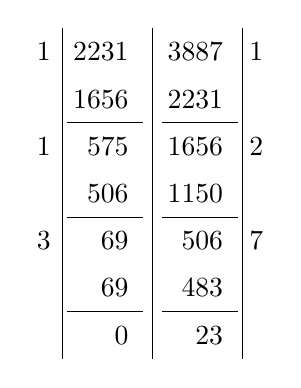
\begin{tikzpicture}[scale=.6]
\foreach \y/\ytext in {0/0,1/69,2/69,3/506,4/575, 5/1656, 6/2231}
{
    \node at (-1, \y)[left]{$\ytext$};
}    
\foreach \y/\ytext in {0/\boxed{23},1/483,2/506,3/1150,4/1656, 5/2231, 6/3887}
{
    \node at (1, \y)[left]{$\ytext$};
}   
\foreach \x in {-2.6,-.7,1.2}
{
    \draw (\x,-.5)--(\x,6.5);
}

\foreach \y in {.5, 2.5, 4.5}
{
    \draw (-2.5,\y)--(-.9,\y);
    \draw (-.5,\y)--(1.1,\y);
}
\node at (-3, 6) {1};
\node at (-3, 4) {1};
\node at (-3, 2) {3};
\node at (1.5, 6) {1};
\node at (1.5, 4) {2};
\node at (1.5, 2) {7};

\end{tikzpicture}
